% 2007 年新课标卷理科第 18 题：三棱锥 S-ABC，O 为 BC 中点。
%   侧面 SAB 与 SAC 为等边三角形，∠BAC=90°；SO 为高（虚线）。
% 来源 PDF：gaokaomath-src/普通高考/2007/2007新课标理(海南,宁夏).pdf
% SHA-256：c8ee1632ac3a7a28aab1150f047a2e1c74398ca2944701e9165237897ae724e2
% 原页：2007新课标理(海南,宁夏).pdf 第 1 页（A3 三栏）第 3 栏，书页码 393。
% 重绘依据：按原页顶点位置、虚实线与 O 点位置重绘。
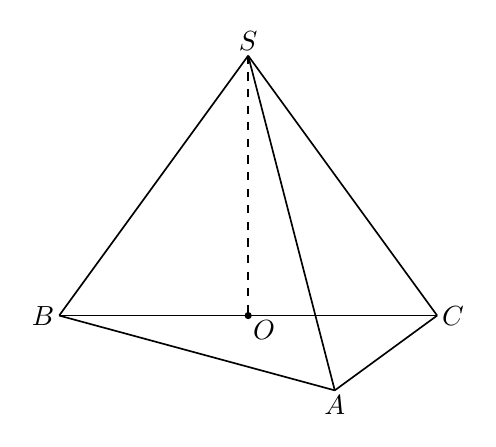
\begin{tikzpicture}[scale=1.0, semithick,
  every node/.style={inner sep=1.5pt}]

  \coordinate (S) at (0,3.3);
  \coordinate (B) at (-2.4,0);
  \coordinate (C) at (2.4,0);
  \coordinate (A) at (1.1,-0.95);
  \coordinate (O) at (0,0);

  \draw (S) -- (A);
  \draw (S) -- (B);
  \draw (S) -- (C);
  \draw (A) -- (B);
  \draw (A) -- (C);
  \draw (B) -- (C);
  \draw[dashed] (S) -- (O);

  \fill (O) circle (1.3pt);
  \node[above] at (S) {$S$};
  \node[left] at (B) {$B$};
  \node[right] at (C) {$C$};
  \node[below] at (A) {$A$};
  \node[below right] at (O) {$O$};
\end{tikzpicture}
